%! Author = bling
%! Date = 2021/12/11

% THIS TEMPLATE IS A WORK IN PROGRESS

\documentclass{article}

\usepackage{hyperref}
\usepackage{fancyhdr}
\usepackage{graphicx}

%\lhead{\includegraphics[width=0.2\textwidth]{nyush-logo.pdf}}
\fancypagestyle{firstpage}{%
  \lhead{NYU Shanghai}
  \rhead{
  %%%% COMMENT OUT / UNCOMMENT THE LINES BELOW TO FIT WITH YOUR MAJOR(S)
  %\&
  %Data
   Machine Learning 2021}
}

%%%% PROJECT TITLE
\title{The Classification of Trash Based on Chinese Trash Polity}

%%%% NAMES OF ALL THE STUDENTS INVOLVED (first-name last-name)
\author{\href{mailto:cw3923@nyu.edu}{Chenyang Wen}, \href{mailto:ct2831@nyu.edu}{Chenyu Tang},
\href{mailto:jg5315@nyu.edu}{Jiacheng Guo}}

\date{\vspace{-5ex}} %NO DATE


\begin{document}
\maketitle
\thispagestyle{firstpage}


\begin{abstract}
    The
    A abstract sums up your work in very few sentences:
    (i) state the problem you are addressing;
    (ii) say why it’s an interesting problem, and which issues are hard to tackle;
    (iii) Compare with three neural networks and choose the best one;
    (iv) say Why and how well your approach solves the problem.
\end{abstract}


\section*{Introduction}
\paragraph{In Shanghai, garbage classification has been implemented for more than 20 years. Meanwhile, the classification standard has changed many times. Published on July 1, 2019, Shanghai Municipal Household Garbage Management Regulations divides the classification standard into four categories: recyclable waste, residual waste, household waste and hazardous waste.  The strict implementation with high quality of garbage classification cannot be separated from the accurate classification by every citizen in Shanghai. In this project, we want to develop a framework to automatic garbage categorization.}

\begin{figure}
    \begin{centering}
    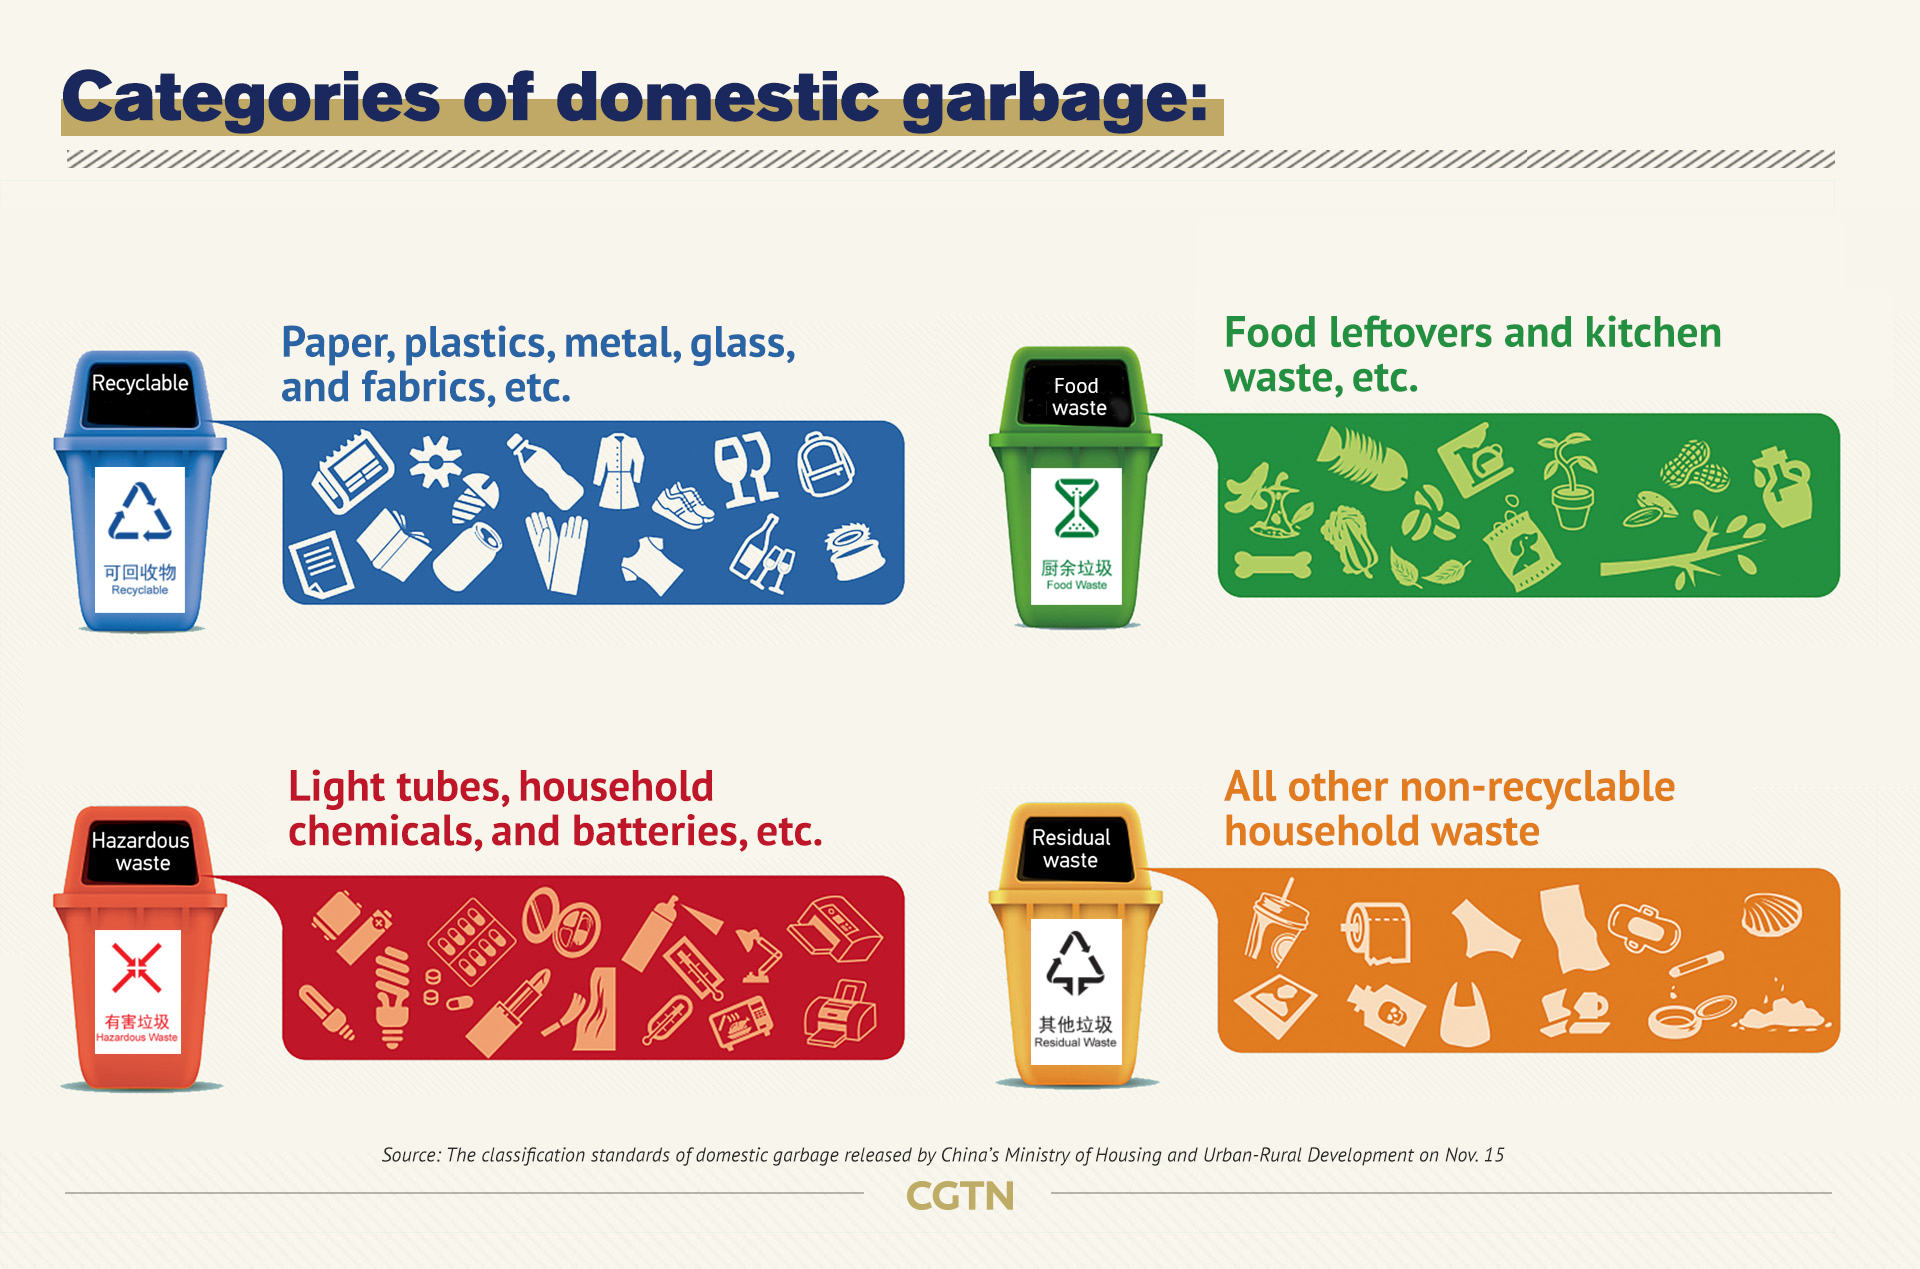
\includegraphics[width=0.95\textwidth]{categories.jpeg}
    \par\end{centering}
    \caption{Standard for waste classification from CGTN}
    \label{fig:Trash_classification}
\end{figure}

\paragraph{Similar to how people identify garbage categories, we also want our framework to be able to output garbage categories when it sees the garbage (i.e., the input image).  The first step in this process requires the ability to recognize the content of the input image. In the field of image identification, machine learning, especially convolutional neural networks, has huge advantages.  After recognizing the image content, our method needs to classify it. Also, there are many classification algorithms in machine learning, with which we hope to achieve good classification performance.}

\paragraph{We have noticed that many papers have made outstanding contributions in the field of image identification, such as gradient-based Learning Applied to Document Recognition, Very Deep Convolutional Networks for large-scale Image Recognition. We will draw on established algorithms to develop this framework for our project.}



\section*{Dataset}

Explain what dataset you will use, and give a short description about the dataset.




\section*{Solution}

Here the project uses

    \subsection*{Data Pre-processing}
    \paragraph{}

    \subsection*{Neural Network \& Model Selection}
    \paragraph{Neural network has already taken a place for many years. Based on the practical experience and experiment result, it performed pretty well, even better than the traditional machine learning algorithm. And the convolutional neural network is one of the main categories to do computer vision tasks both in recognition and classification. Since the project is based on the image classification, the most common way to classify the image for now is to use deep neural network. And this is also the most mature way in computer vision, so we here specify three different network for training.}
    \paragraph{The basic CNN with 2 convolution layers and 3 fully connected layers that for trash classification tasks is as the base line for the improvement of other models. And compare with the basic CNN, wasteCNN add one convolutional layer addition for improvement; and another neural network is Res18, cascading with previous layers. This kind of skip connection let the ResNet able to preserve the feature from previous layers, make the network much easier to preserve the gradient.}


    \subsection*{Choose Models to Compare \& Training}
    \paragraph{And as for the model chosen process, because if the model is much deeper, then the time consuming for training process will be much longer, so the res18 is the deepest network we choose. It is true that the Res50 will have much deeper network and similar amount of parameter for the network (or in other work the size of the network), it is also the network we want to realize by ourselves, but these are sufficient to classify the trash by these models and choose the best one. }

        \subsubsection*{CNN}
        \paragraph{Figure \ref{fig:cnn_model} show the model structure with the image size is 128, adjusting the image size will affect the model’s first fully connected layer.}
        \begin{figure}
            \begin{centering}
            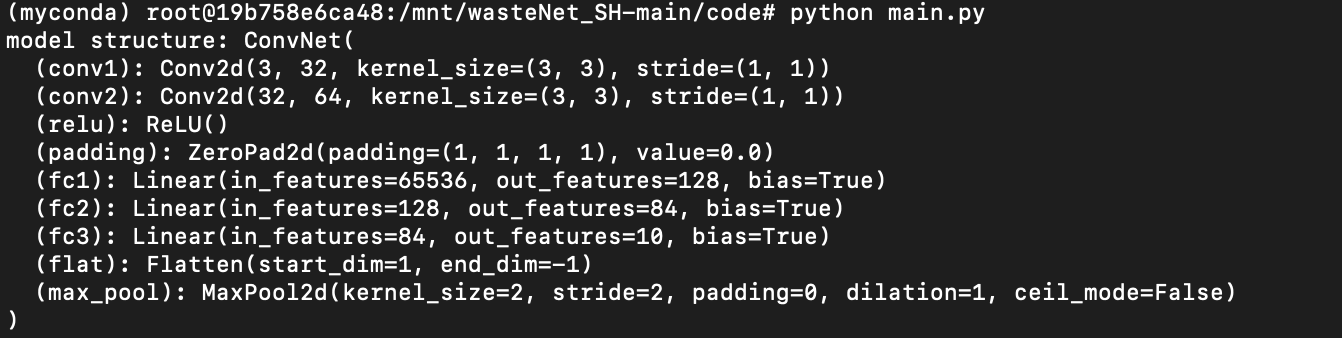
\includegraphics[width=0.95\textwidth]{CNN.png}
            \par\end{centering}
            \caption{Convolutional Neural Network structure}
            \label{fig:cnn_model}
        \end{figure}

        \subsubsection*{WasteCNN}
        \paragraph{The model structure is shown in Figure \ref{fig:wasteNet_model} with the image size is 128, adjusting the image size will affect the model’s first fully connected layer. Basic backbone is as same as CNN. The difference is that there is 3 convolutional layers and larger fully connected layer.}
        \begin{figure}
            \begin{centering}
            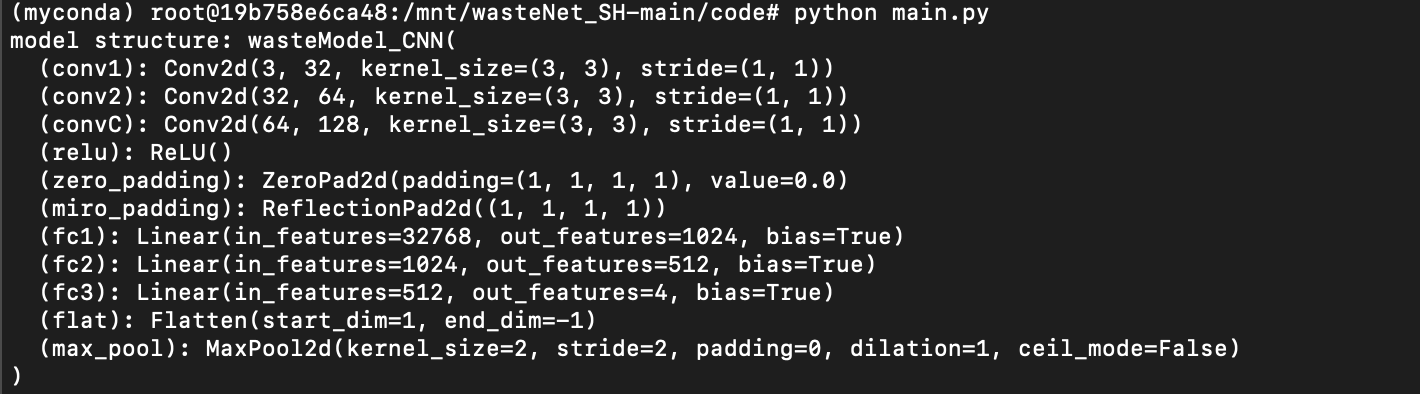
\includegraphics[width=0.95\textwidth]{wasteCNN.png}
            \par\end{centering}
            \caption{wasteCNN model structure}
            \label{fig:wasteNet_model}
        \end{figure}

        \subsubsection*{Res18}
        \paragraph{Res18 has 18 convolutional layers. First thing is to construct the ResBlock, which is the basic component for the ResNet. ResBlock is built by two convolutional layers and a shortcut, which represent the combination of current Conv layer output and previous output. Then connect with 4 blocks and addition 1 conv-layer in the front and 1 fully connected layer at the end. And the part of ResNet is also shown as Figure \ref{fig:res18_model}}
        \begin{figure}
            \begin{centering}
            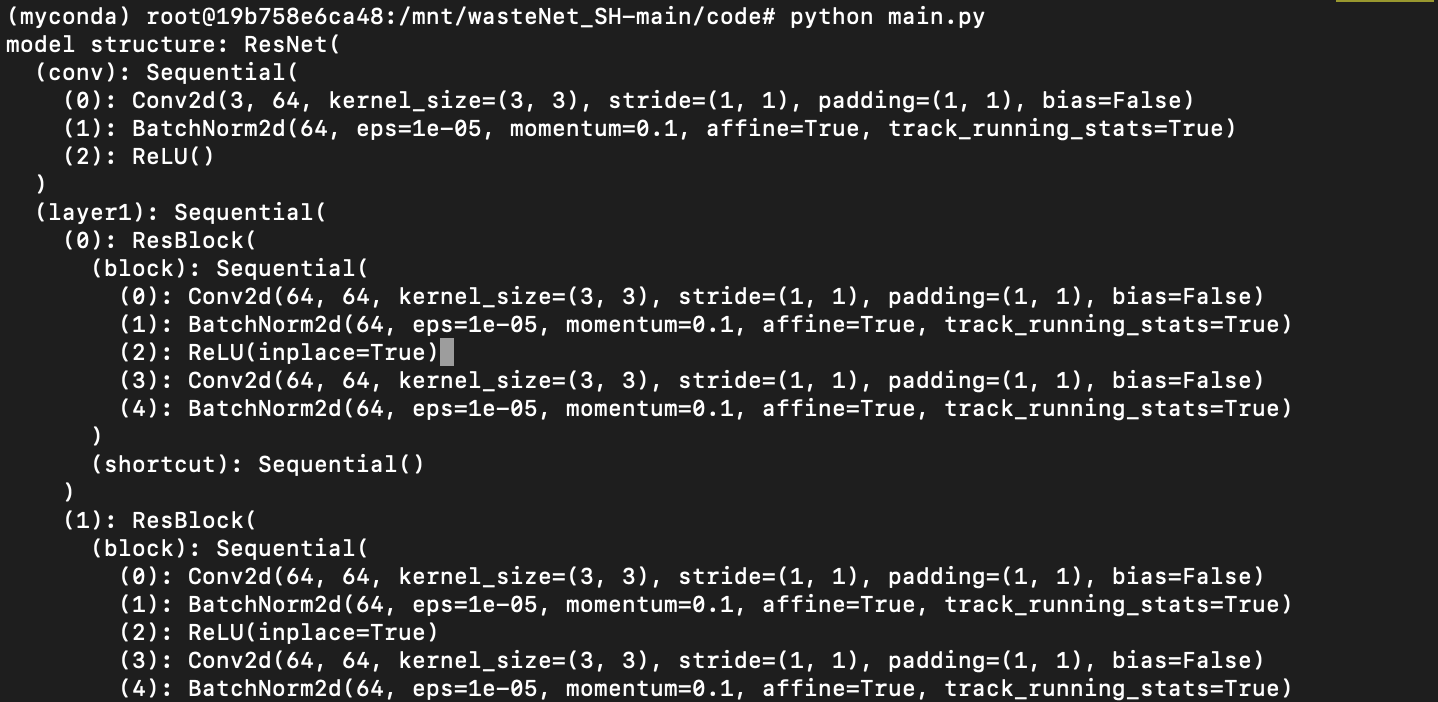
\includegraphics[width=0.95\textwidth]{Res18.png}
            \par\end{centering}
            \caption{Part of ResNet with 18 convolutional layer}
            \label{fig:res18_model}
        \end{figure}


\section*{Results and Discussion}
\paragraph{The project separately evaluates these three kinds of models by using many evaluation methods and obtained the following figures and results: the variation curve of Test Accuracy with the number of epochs shown as Figure \ref{fig:Accuracy}. And the variation curve of AUC value with the number of epochs as Figure \ref{fig:AUC}.}

\begin{figure}
    \begin{centering}
    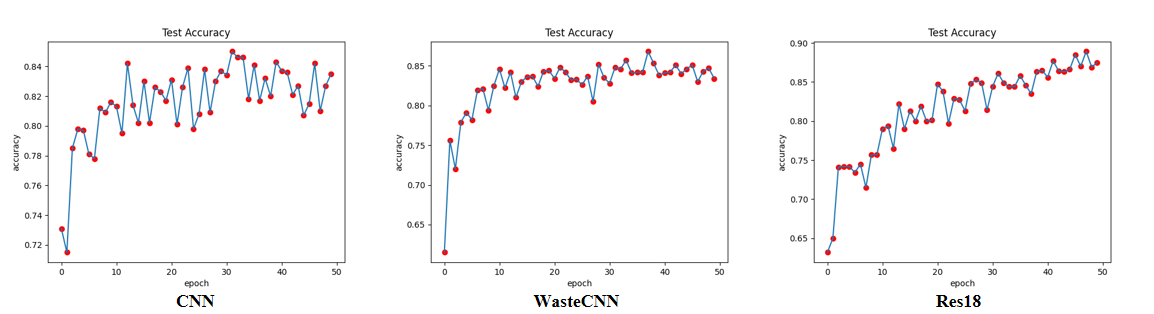
\includegraphics[width=0.95\textwidth]{accuracy.png}
    \par\end{centering}
    \caption{Accuracy-Epoch Curve}
    \label{fig:Accuracy}
\end{figure}

\begin{figure}
    \begin{centering}
    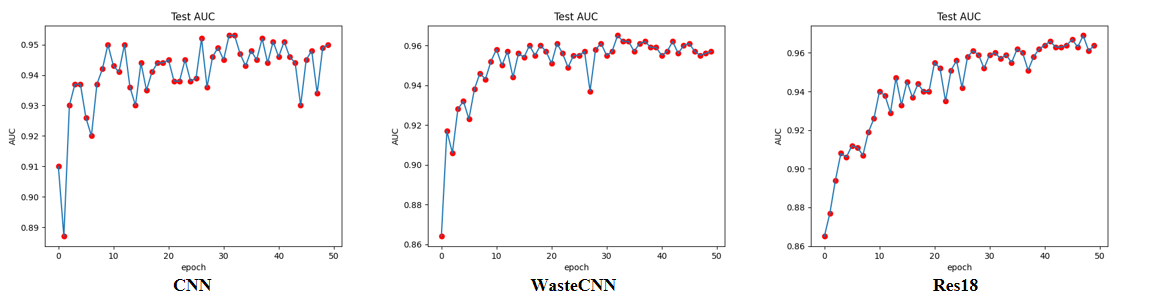
\includegraphics[width=0.95\textwidth]{AUC.png}
    \par\end{centering}
    \caption{AUC value-Epoch Curve}
    \label{fig:AUC}
\end{figure}

\paragraph{According to figures 6 and 7, the project selects the iteration that performs better in the test dataset and get the confusion matrix and ROC curve (after averaging the four categories) under that iteration. Then calculate the Precision, Recall for each category.}

\paragraph{Due to the uneven distribution of data in the test set, the project decides to calculate the macro average and micro average of precision, recall and F1-score of the three models respectively to compare the performance.}

\begin{figure}
    \begin{centering}
    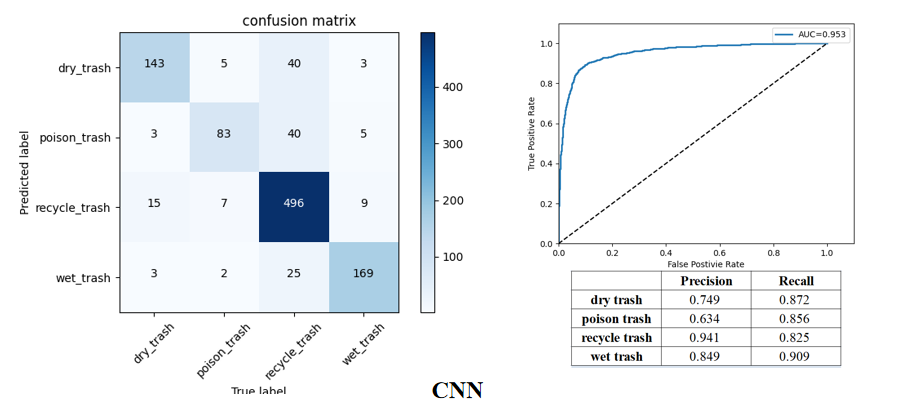
\includegraphics[width=0.95\textwidth]{CNN_eva.png}
    \par\end{centering}
    \caption{Confusion metrics and ROC curves of CNN}
    \label{fig:CNN_confusion_ROC}
\end{figure}

\begin{figure}
    \begin{centering}
    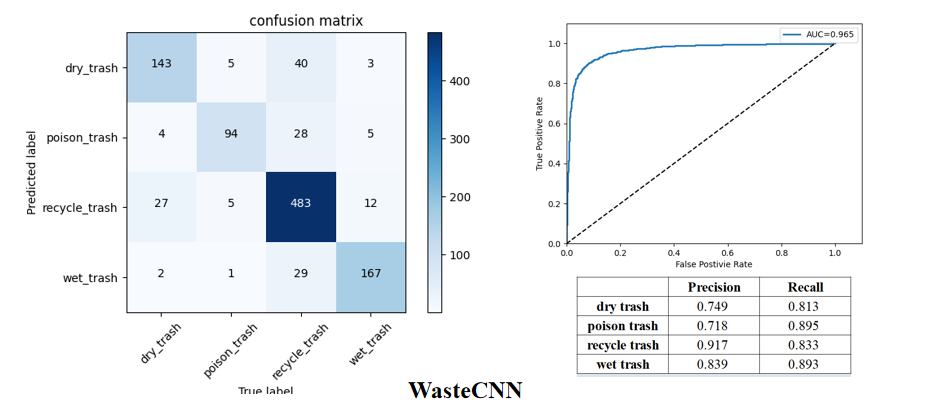
\includegraphics[width=0.95\textwidth]{WasteCNN_eva.png}
    \par\end{centering}
    \caption{Confusion metrics and ROC curves of WasteCNN}
    \label{fig:WasteCNN_confusion_ROC}
\end{figure}

\begin{figure}
    \begin{centering}
    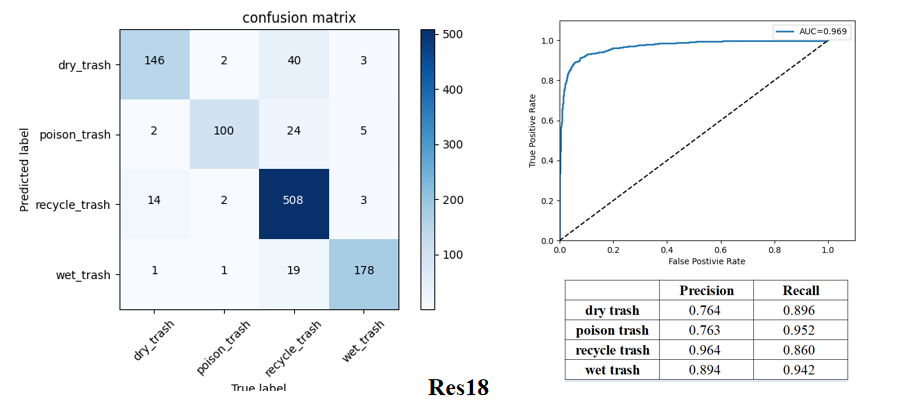
\includegraphics[width=0.95\textwidth]{Res18_eva.png}
    \par\end{centering}
    \caption{Confusion metrics and ROC curves of Res18}
    \label{fig:Res18_confusion_ROC}
\end{figure}

\begin{table}[]
    \centering
    \begin{tabular}{ |p{2cm}||p{2cm}|p{2cm}|p{2cm}|  }
        \hline
            \multicolumn{4}{|c|}{Macro average} \\
        \hline
             & Precision &Recall&F1-score\\
        \hline
            CNN    &   0.793   &   0.865  &    0.828\\
            WasteCNN    &   0.805   &   0.858   &   0.831\\
            Res18   &   0.847   &   0.912   &   0.878\\
        \hline\hline
            \multicolumn{4}{|c|}{Micro average} \\
        \hline
             & Precision &Recall&F1-score\\
        \hline
            CNN    &   0.850   &   0.850  &    0.850\\
            WasteCNN    &   0.846   &   0.846   &   0.846\\
            Res18   &   0.889   &   0.889   &   0.889\\
        \hline
    \end{tabular}
    \caption{Value of precision, recall and F1-score}
    \label{tab:my_label}
\end{table}

\paragraph{These results shows that Res18 model has the highest accuracy when predicting the test dataset, accuracy is up to 89\% within 50 iterations, while the accuracy of CNN and wasteCNN models is about 83\% and 85\%. In addition, the average Precision, Recall and F1-score values of the Res18 model are also the closest to "1". The Precision, Recall and F1-score calculated by macro and micro average methods are basically the same, indicating the accuracy of classification is not affected by the number of samples in different categories. The AUC value of Res18 model is up to 0.97 within 50 iterations, which is also higher than in the wasteCNN and CNN models. Hence, it can be seen that Res18 model is the most accurate in the classification of trash pictures among these three models.}

\paragraph{However, in the case of calculating the values of precision and recall by category of garbage, the classification accuracy of the three models is the highest for recyclable trash, which is up to 96\%, but lower for dry trash and poison trash categories. This problem needs further study.}

\nocite{*}
\bibliographystyle{IEEEtran}
\bibliography{references}



\end{document}
